\section{Methodology}
\label{sec:method}

\begin{figure*}[t]
  \centering
  
\includegraphics[width=1\linewidth, trim=0 170 0 55, clip]{figs/pipeline.png}

  \label{fig:pipeline}
\end{figure*}

Our goal is to directly predict a clean 3D Gaussian scene representation and its renderings from noisy multi-view inputs. The overall pipeline is illustrated in Fig.~2. We first construct multi-noise-type noisy--clean paired multi-view data based on RE10K. Then, we design a feed-forward Gaussian splatting network on top of the MVSplat framework, which takes noisy images as input and is trained end-to-end with clean renderings as supervision. At test time, a single forward pass suffices to obtain a clean 3DGS scene and high-quality novel views.

\subsection{Problem Definition and Overall Pipeline}
\label{subsec:problem_overview}

Given a collection of 3D scenes
\(
\mathcal{S} = \{s\}
\),
each scene \(s\) provides \(V\) clean images
\(
\{I^{\text{GT}}_{s,v}\}_{v=1}^{V}
\)
with corresponding camera parameters
\(
\{\mathcal{C}_{s,v}\}_{v=1}^{V}
\).
Following the noise degradation process in Sec.~\ref{subsec:noise_degradation_dataset}, we synthetically generate noisy observations by applying a 2D RGB-domain corruption operator \(\mathcal{D}(\cdot)\) to each clean image while keeping the viewpoints unchanged:
\begin{equation}
\bigl\{\tilde{I}^{\text{noise}}_{s,v},\, I^{\text{GT}}_{s,v},\, \mathcal{C}_{s,v}\bigr\}_{v=1}^{V},
\qquad
\tilde{I}^{\text{noise}}_{s,v}=\mathcal{D}\!\left(I^{\text{GT}}_{s,v}\right).
\end{equation}
Here \(\tilde{I}^{\text{noise}}_{s,v}\) denotes the noisy image obtained in the 2D RGB domain; the camera parameters and underlying scene geometry are shared with the corresponding clean view by construction.

Our goal is to learn parameters \(\theta\) of a feed-forward predictor that maps multi-view noisy observations (and cameras) to a 3D Gaussian scene representation and its renderings:
\begin{equation}
f_{\theta}:\ 
\bigl(\{\tilde{I}^{\text{noise}}_{s,v}\}_{v=1}^{V}, \{\mathcal{C}_{s,v}\}_{v=1}^{V}\bigr)
\;\longrightarrow\;
\bigl(\mathcal{G}_{s}, \{\hat{I}_{s,v}\}_{v=1}^{V}\bigr),
\end{equation}
where \(\mathcal{G}_{s}\) is the reconstructed 3D scene represented by Gaussian primitives, and \(\hat{I}_{s,v}\) is rendered from \(\mathcal{G}_{s}\) under \(\mathcal{C}_{s,v}\).
During training, we use only 2D image-domain supervision by comparing \(\hat{I}_{s,v}\) with \(I^{\text{GT}}_{s,v}\).
At test time, the clean images are not available; the model predicts \(\mathcal{G}_{s}\) and \(\hat{I}_{s,v}\) \emph{conditioned on} noisy multi-view inputs and camera parameters in a single forward pass.


\subsection{Noise Degradation and Dataset Construction}
\label{subsec:noise_degradation_dataset}

\textbf{Modeling multiple noise types.}
We build our noisy multi-view benchmark on top of the RealEstate10K (RE10K) dataset~\cite{realestate10k}, which contains camera trajectories for approximately 80{,}000 video clips collected from around 10{,}000 YouTube real-estate videos, 
totalling about 10 million frames. For each clip, the dataset provides a sequence of calibrated camera poses along a viewing trajectory, making it a standard testbed for novel view synthesis and 3D scene reconstruction. Starting from the original clean multi-view RE10K data, we synthesize four common noise types in the 2D RGB image domain:
Gaussian noise, Poisson noise, speckle noise, and salt-and-pepper noise. Let
\(
I \in [0,1]^{H\times W \times 3}
\)
denote an input normalized image and \(\tilde{I}\) the degraded one. The four noise types can be summarized as:
\begin{itemize}
    \item Gaussian noise: \(\tilde{I} = \mathrm{clip}(I + \mathcal{N}(0,\sigma^{2}))\);
    \item Poisson noise: \(\tilde{I} = \mathrm{clip}\bigl(s \cdot \mathrm{Poisson}(I/s)\bigr)\);
    \item Speckle noise: \(\tilde{I} = \mathrm{clip}\bigl(I + I \odot \mathcal{N}(0,\sigma^{2})\bigr)\);
    \item Salt-and-pepper noise: each pixel is set to 0 or 1 with probability \(\alpha\).
\end{itemize}
Here \(\sigma\) or \(\alpha\) is uniformly sampled within a predefined range, e.g., the standard deviation of Gaussian noise is sampled from \([0.08, 0.12]\), and the total ratio of salt-and-pepper noise is sampled from \([0.015, 0.03]\). All specific values are managed through a unified configuration file in our implementation.

\noindent \textbf{Scene-level noise configuration.}
In practice, images from the same scene are typically captured with the same device and exposure settings, so their noise types and strengths tend to be consistent across views. To reflect this, we adopt a scene-level noise sampling strategy. For each scene \(s\):
\begin{enumerate}
    \item uniformly sample a noise type \(t_{s}\) from the four candidates;
    \item sample a noise parameter \(\phi_{s}\) within the intensity range corresponding to type \(t_{s}\);
    \item apply the same pair \((t_{s}, \phi_{s})\) to all views \(\{v\}\) of that scene.
\end{enumerate}
The resulting noisy--clean multi-view data thus maintains noise consistency at the scene level while exhibiting diversity across scenes. All noise configurations (types and strengths) are recorded in a separate metadata file to facilitate reproducibility and ablation studies.




\subsection{Feed-forward Gaussian Splatting Network}
\label{subsec:ff_gs_network}

\noindent \textbf{Gaussian scene representation and rendering.}
We follow 3DGS~\cite{kerbl3Dgaussians} and represent a scene \(s\) as a set of Gaussian primitives
\begin{equation}
\mathcal{G}_{s} = \{g_{i}\}_{i=1}^{N},\quad
g_{i} = (\mathbf{x}_{i}, \Sigma_{i}, \alpha_{i}, \mathbf{c}_{i}),
\end{equation}
where \(\mathbf{x}_{i} \in \mathbb{R}^{3}\) is the center position, \(\Sigma_{i} \in \mathbb{R}^{3\times 3}\) is the covariance matrix, \(\alpha_{i} \in [0,1]\) is the opacity, and \(\mathbf{c}_{i}\) denotes the appearance parameters (spherical-harmonics coefficients plus a base color).
Given camera parameters \(\mathcal{C}_{s,v}\) for view \(v\), a differentiable Gaussian splatting renderer \(\mathcal{R}\) produces
\begin{equation}
\hat{I}_{s,v} = \mathcal{R}(\mathcal{G}_{s}, \mathcal{C}_{s,v}) \in \mathbb{R}^{H\times W\times 3}.
\end{equation}

\noindent \textbf{MVSplat-based feed-forward architecture.}
Our network is built on the feed-forward design of MVSplat~\cite{chen2024mvsplat}: a shared multi-view 2D encoder extracts per-view features, which are then lifted and aggregated in a geometry-aligned manner to form a unified 3D representation (Fig.~2).
Concretely, the pipeline consists of three stages:

\begin{itemize}
    \item \textbf{Multi-view feature encoding.}
    For each noisy view \(\tilde{I}^{\text{noise}}_{s,v}\), a shared-weight 2D convolutional encoder produces multi-scale feature maps \(\{\mathbf{F}^{(l)}_{s,v}\}_{l=1}^{L}\).
    Rather than explicitly outputting a denoised image, the encoder learns feature representations that retain task-relevant structures while being tolerant to noise, under the downstream reconstruction objective.

    \item \textbf{Geometry-aligned 3D aggregation.}
    Conditioned on camera parameters \(\mathcal{C}_{s,v}\), we follow MVSplat and warp multi-view features into a plane-sweep volume via differentiable homography projection over discrete depth planes.
    The resulting 3D feature volume \(\mathbf{F}^{3\mathrm{D}}_{s}\) encodes multi-view consistency signals and serves as the input to the Gaussian prediction head.

    \item \textbf{Dual-branch Gaussian parameter prediction.}
    Different from the single shared head in MVSplat, we adopt a \emph{dual-branch Gaussian head} tailored for noisy inputs.
    The aggregated features \(\mathbf{F}^{3\mathrm{D}}_{s}\) are fed into two lightweight decoupled branches:
    (1) a \textbf{geometry branch} that predicts centers \(\mathbf{x}_{i}\), rotations, scales, and opacities \(\alpha_{i}\), and
    (2) an \textbf{appearance branch} that predicts spherical-harmonics coefficients and colors \(\mathbf{c}_{i}\).
    This decoupling is a modeling choice that allows the geometry branch to prioritize relatively stable structural cues, while the appearance branch can account for residual noise and color fluctuations.
    Empirically, this design improves structural consistency and texture sharpness across varying noise types and intensities.
\end{itemize}

\noindent \textbf{2D rendering supervision and loss functions.}
During training, we supervise reconstruction only in the 2D image domain by comparing \(\hat{I}_{s,v}\) with \(I^{\text{GT}}_{s,v}\).
We use a combination of pixel-wise \(\ell_{1}\) loss and structural similarity (SSIM):
\begin{equation}
\mathcal{L}
= \sum_{s}\sum_{v}
\bigl(
\lambda_{1}\,\lVert \hat{I}_{s,v} - I^{\text{GT}}_{s,v} \rVert_{1}
+ \lambda_{2}\,\bigl(1 - \mathrm{SSIM}(\hat{I}_{s,v}, I^{\text{GT}}_{s,v})\bigr)
\bigr),
\label{eq:reconstruction_loss}
\end{equation}
where \(\lambda_{1}\) and \(\lambda_{2}\) are weighting coefficients.
The loss is averaged over pixels within each view and summed over training scenes and views.

After end-to-end training on the noisy--clean paired data (Sec.~\ref{subsec:noise_degradation_dataset}), the model learns to predict a Gaussian scene representation whose renderings match the clean targets under the above objective.
At test time, given only noisy multi-view inputs, a single forward pass through DenoiseSplat outputs \(\mathcal{G}_{s}\) and corresponding renderings, without test-time optimization or an external 2D denoiser.



\subsection{Cross-Branch Boundary-Guided Appearance Correction (CBC)}
\label{subsec:cbc}

Our dual-branch design decouples geometry and appearance to improve robustness under noisy inputs, yet appearance estimation may still degrade when the geometry branch is uncertain, especially near geometric boundaries (e.g., depth/disparity discontinuities and occlusion edges).
In such regions, even small geometric inaccuracies can coincide with perceptually salient artifacts after rendering.
To mitigate this \emph{cross-branch error propagation} in a controlled manner, we introduce a lightweight \emph{cross-branch correction mechanism}, termed \textbf{CBC}, which leverages geometry-derived boundary strength and confidence as \emph{conditional signals} to gate a residual refinement in the appearance branch.

\noindent\textbf{Geometry-conditioned boundary gating.}
We construct a boundary-guided gating map from the full-resolution disparity (or depth) predicted by the geometry branch, together with a confidence proxy derived from the candidate distribution over disparity/depth hypotheses (e.g., obtained by applying \(\mathrm{softmax}\) to the cost-volume logits along the plane dimension).
Using disparity $\delta$ for clarity, we compute
\begin{equation}
E = \left\lVert \nabla \delta \right\rVert,\quad
C = \max(\mathrm{pdf}),\quad
B = \operatorname{norm}(E)\cdot(1-C),
\label{eq:cbc_gate}
\end{equation}
where $E$ denotes boundary strength (the gradient magnitude of $\delta$), and $C$ is the maximum probability of the disparity/depth candidate distribution $\mathrm{pdf}$ as a confidence proxy.
The resulting $B\in[0,1]$ emphasizes regions that are simultaneously boundary-like and low-confidence: $B$ increases when $E$ is strong and $C$ is small.

\noindent\textbf{Boundary-guided residual correction in appearance.}
Let $A$ denote the output of the appearance branch (e.g., SH/color-related parameters or logits).
CBC predicts a residual correction $\Delta A$ via a lightweight CNN $g(\cdot)$ conditioned on $(A,B,C)$:
\begin{equation}
\Delta A = g([A, B, C]),\quad
A' = A + B \odot \Delta A,
\label{eq:cbc_residual}
\end{equation}
where $[\cdot]$ denotes channel-wise concatenation and $\odot$ is the element-wise product.
This design applies refinement primarily where $B$ is large, thereby suppressing boundary artifacts while avoiding unnecessary modification in non-boundary or high-confidence regions.

\noindent\textbf{Implementation detail (gradient isolation).}
During training, we apply stop-gradient to the geometry-derived signals by detaching $B$ and $C$ (i.e., \texttt{detach}).
As a result, CBC updates only the appearance-branch parameters and the CBC module parameters, preventing appearance gradients from back-propagating into the geometry branch.
This realizes an explicit cross-branch interaction mechanism: geometry provides conditional boundary/confidence cues, and appearance performs a gated residual refinement accordingly.
We provide qualitative evidence of CBC in Fig.~3.

\begin{figure}[ht]
    \centering
    \label{cbc_zoom}
    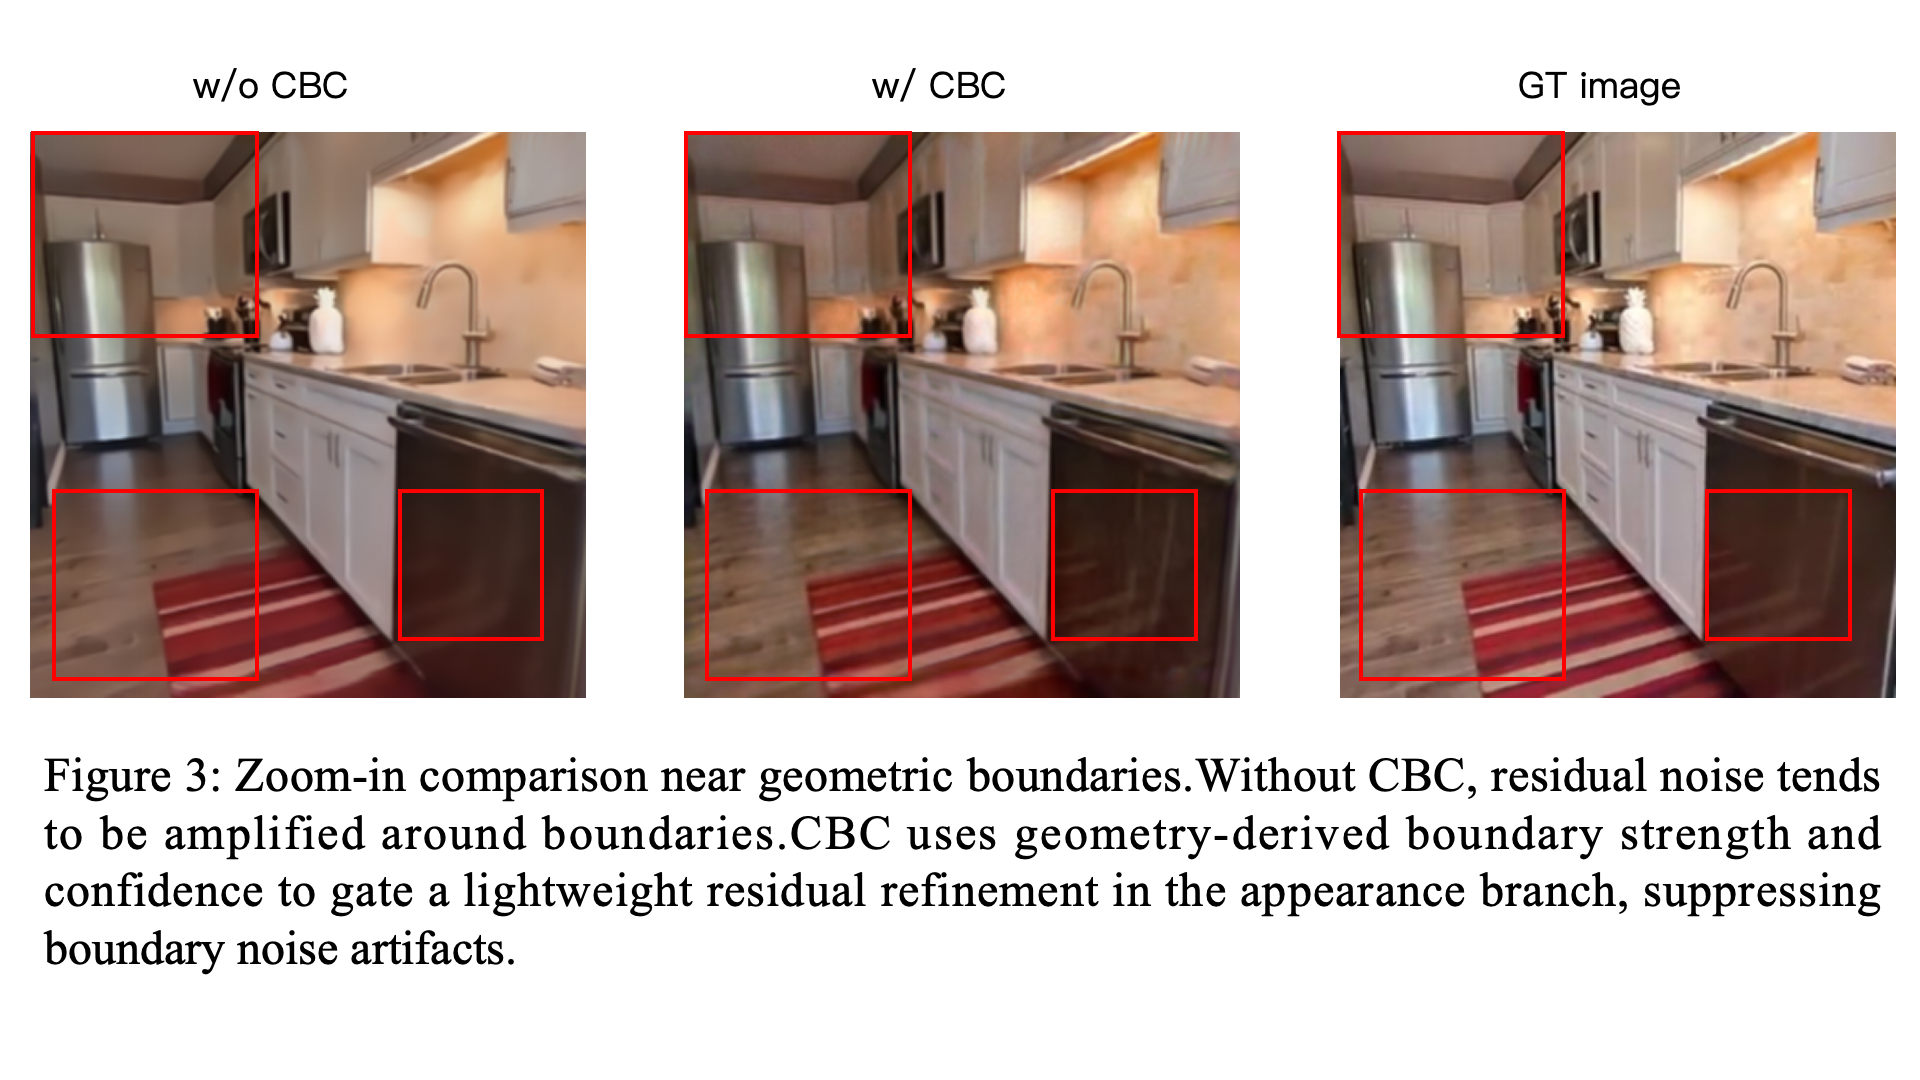
\includegraphics[width=1\linewidth, trim=0 100 0 0, clip]{figs/cbc_zoom.png}
\end{figure}
